\documentclass[11pt]{article}

    \usepackage[breakable]{tcolorbox}
    \usepackage{parskip} % Stop auto-indenting (to mimic markdown behaviour)
    
    \usepackage{iftex}
    \ifPDFTeX
    	\usepackage[T1]{fontenc}
    	\usepackage{mathpazo}
    \else
    	\usepackage{fontspec}
    \fi

    % Basic figure setup, for now with no caption control since it's done
    % automatically by Pandoc (which extracts ![](path) syntax from Markdown).
    \usepackage{graphicx}
    % Maintain compatibility with old templates. Remove in nbconvert 6.0
    \let\Oldincludegraphics\includegraphics
    % Ensure that by default, figures have no caption (until we provide a
    % proper Figure object with a Caption API and a way to capture that
    % in the conversion process - todo).
    \usepackage{caption}
    \DeclareCaptionFormat{nocaption}{}
    \captionsetup{format=nocaption,aboveskip=0pt,belowskip=0pt}

    \usepackage{float}
    \floatplacement{figure}{H} % forces figures to be placed at the correct location
    \usepackage{xcolor} % Allow colors to be defined
    \usepackage{enumerate} % Needed for markdown enumerations to work
    \usepackage{geometry} % Used to adjust the document margins
    \usepackage{amsmath} % Equations
    \usepackage{amssymb} % Equations
    \usepackage{textcomp} % defines textquotesingle
    % Hack from http://tex.stackexchange.com/a/47451/13684:
    \AtBeginDocument{%
        \def\PYZsq{\textquotesingle}% Upright quotes in Pygmentized code
    }
    \usepackage{upquote} % Upright quotes for verbatim code
    \usepackage{eurosym} % defines \euro
    \usepackage[mathletters]{ucs} % Extended unicode (utf-8) support
    \usepackage{fancyvrb} % verbatim replacement that allows latex
    \usepackage{grffile} % extends the file name processing of package graphics 
                         % to support a larger range
    \makeatletter % fix for old versions of grffile with XeLaTeX
    \@ifpackagelater{grffile}{2019/11/01}
    {
      % Do nothing on new versions
    }
    {
      \def\Gread@@xetex#1{%
        \IfFileExists{"\Gin@base".bb}%
        {\Gread@eps{\Gin@base.bb}}%
        {\Gread@@xetex@aux#1}%
      }
    }
    \makeatother
    \usepackage[Export]{adjustbox} % Used to constrain images to a maximum size
    \adjustboxset{max size={0.9\linewidth}{0.9\paperheight}}

    % The hyperref package gives us a pdf with properly built
    % internal navigation ('pdf bookmarks' for the table of contents,
    % internal cross-reference links, web links for URLs, etc.)
    \usepackage{hyperref}
    % The default LaTeX title has an obnoxious amount of whitespace. By default,
    % titling removes some of it. It also provides customization options.
    \usepackage{titling}
    \usepackage{longtable} % longtable support required by pandoc >1.10
    \usepackage{booktabs}  % table support for pandoc > 1.12.2
    \usepackage[inline]{enumitem} % IRkernel/repr support (it uses the enumerate* environment)
    \usepackage[normalem]{ulem} % ulem is needed to support strikethroughs (\sout)
                                % normalem makes italics be italics, not underlines
    \usepackage{mathrsfs}
    

    
    % Colors for the hyperref package
    \definecolor{urlcolor}{rgb}{0,.145,.698}
    \definecolor{linkcolor}{rgb}{.71,0.21,0.01}
    \definecolor{citecolor}{rgb}{.12,.54,.11}

    % ANSI colors
    \definecolor{ansi-black}{HTML}{3E424D}
    \definecolor{ansi-black-intense}{HTML}{282C36}
    \definecolor{ansi-red}{HTML}{E75C58}
    \definecolor{ansi-red-intense}{HTML}{B22B31}
    \definecolor{ansi-green}{HTML}{00A250}
    \definecolor{ansi-green-intense}{HTML}{007427}
    \definecolor{ansi-yellow}{HTML}{DDB62B}
    \definecolor{ansi-yellow-intense}{HTML}{B27D12}
    \definecolor{ansi-blue}{HTML}{208FFB}
    \definecolor{ansi-blue-intense}{HTML}{0065CA}
    \definecolor{ansi-magenta}{HTML}{D160C4}
    \definecolor{ansi-magenta-intense}{HTML}{A03196}
    \definecolor{ansi-cyan}{HTML}{60C6C8}
    \definecolor{ansi-cyan-intense}{HTML}{258F8F}
    \definecolor{ansi-white}{HTML}{C5C1B4}
    \definecolor{ansi-white-intense}{HTML}{A1A6B2}
    \definecolor{ansi-default-inverse-fg}{HTML}{FFFFFF}
    \definecolor{ansi-default-inverse-bg}{HTML}{000000}

    % common color for the border for error outputs.
    \definecolor{outerrorbackground}{HTML}{FFDFDF}

    % commands and environments needed by pandoc snippets
    % extracted from the output of `pandoc -s`
    \providecommand{\tightlist}{%
      \setlength{\itemsep}{0pt}\setlength{\parskip}{0pt}}
    \DefineVerbatimEnvironment{Highlighting}{Verbatim}{commandchars=\\\{\}}
    % Add ',fontsize=\small' for more characters per line
    \newenvironment{Shaded}{}{}
    \newcommand{\KeywordTok}[1]{\textcolor[rgb]{0.00,0.44,0.13}{\textbf{{#1}}}}
    \newcommand{\DataTypeTok}[1]{\textcolor[rgb]{0.56,0.13,0.00}{{#1}}}
    \newcommand{\DecValTok}[1]{\textcolor[rgb]{0.25,0.63,0.44}{{#1}}}
    \newcommand{\BaseNTok}[1]{\textcolor[rgb]{0.25,0.63,0.44}{{#1}}}
    \newcommand{\FloatTok}[1]{\textcolor[rgb]{0.25,0.63,0.44}{{#1}}}
    \newcommand{\CharTok}[1]{\textcolor[rgb]{0.25,0.44,0.63}{{#1}}}
    \newcommand{\StringTok}[1]{\textcolor[rgb]{0.25,0.44,0.63}{{#1}}}
    \newcommand{\CommentTok}[1]{\textcolor[rgb]{0.38,0.63,0.69}{\textit{{#1}}}}
    \newcommand{\OtherTok}[1]{\textcolor[rgb]{0.00,0.44,0.13}{{#1}}}
    \newcommand{\AlertTok}[1]{\textcolor[rgb]{1.00,0.00,0.00}{\textbf{{#1}}}}
    \newcommand{\FunctionTok}[1]{\textcolor[rgb]{0.02,0.16,0.49}{{#1}}}
    \newcommand{\RegionMarkerTok}[1]{{#1}}
    \newcommand{\ErrorTok}[1]{\textcolor[rgb]{1.00,0.00,0.00}{\textbf{{#1}}}}
    \newcommand{\NormalTok}[1]{{#1}}
    
    % Additional commands for more recent versions of Pandoc
    \newcommand{\ConstantTok}[1]{\textcolor[rgb]{0.53,0.00,0.00}{{#1}}}
    \newcommand{\SpecialCharTok}[1]{\textcolor[rgb]{0.25,0.44,0.63}{{#1}}}
    \newcommand{\VerbatimStringTok}[1]{\textcolor[rgb]{0.25,0.44,0.63}{{#1}}}
    \newcommand{\SpecialStringTok}[1]{\textcolor[rgb]{0.73,0.40,0.53}{{#1}}}
    \newcommand{\ImportTok}[1]{{#1}}
    \newcommand{\DocumentationTok}[1]{\textcolor[rgb]{0.73,0.13,0.13}{\textit{{#1}}}}
    \newcommand{\AnnotationTok}[1]{\textcolor[rgb]{0.38,0.63,0.69}{\textbf{\textit{{#1}}}}}
    \newcommand{\CommentVarTok}[1]{\textcolor[rgb]{0.38,0.63,0.69}{\textbf{\textit{{#1}}}}}
    \newcommand{\VariableTok}[1]{\textcolor[rgb]{0.10,0.09,0.49}{{#1}}}
    \newcommand{\ControlFlowTok}[1]{\textcolor[rgb]{0.00,0.44,0.13}{\textbf{{#1}}}}
    \newcommand{\OperatorTok}[1]{\textcolor[rgb]{0.40,0.40,0.40}{{#1}}}
    \newcommand{\BuiltInTok}[1]{{#1}}
    \newcommand{\ExtensionTok}[1]{{#1}}
    \newcommand{\PreprocessorTok}[1]{\textcolor[rgb]{0.74,0.48,0.00}{{#1}}}
    \newcommand{\AttributeTok}[1]{\textcolor[rgb]{0.49,0.56,0.16}{{#1}}}
    \newcommand{\InformationTok}[1]{\textcolor[rgb]{0.38,0.63,0.69}{\textbf{\textit{{#1}}}}}
    \newcommand{\WarningTok}[1]{\textcolor[rgb]{0.38,0.63,0.69}{\textbf{\textit{{#1}}}}}
    
    
    % Define a nice break command that doesn't care if a line doesn't already
    % exist.
    \def\br{\hspace*{\fill} \\* }
    % Math Jax compatibility definitions
    \def\gt{>}
    \def\lt{<}
    \let\Oldtex\TeX
    \let\Oldlatex\LaTeX
    \renewcommand{\TeX}{\textrm{\Oldtex}}
    \renewcommand{\LaTeX}{\textrm{\Oldlatex}}
    % Document parameters
    % Document title
    \title{BF18.17}
    
    
    
    
    
% Pygments definitions
\makeatletter
\def\PY@reset{\let\PY@it=\relax \let\PY@bf=\relax%
    \let\PY@ul=\relax \let\PY@tc=\relax%
    \let\PY@bc=\relax \let\PY@ff=\relax}
\def\PY@tok#1{\csname PY@tok@#1\endcsname}
\def\PY@toks#1+{\ifx\relax#1\empty\else%
    \PY@tok{#1}\expandafter\PY@toks\fi}
\def\PY@do#1{\PY@bc{\PY@tc{\PY@ul{%
    \PY@it{\PY@bf{\PY@ff{#1}}}}}}}
\def\PY#1#2{\PY@reset\PY@toks#1+\relax+\PY@do{#2}}

\expandafter\def\csname PY@tok@w\endcsname{\def\PY@tc##1{\textcolor[rgb]{0.73,0.73,0.73}{##1}}}
\expandafter\def\csname PY@tok@c\endcsname{\let\PY@it=\textit\def\PY@tc##1{\textcolor[rgb]{0.25,0.50,0.50}{##1}}}
\expandafter\def\csname PY@tok@cp\endcsname{\def\PY@tc##1{\textcolor[rgb]{0.74,0.48,0.00}{##1}}}
\expandafter\def\csname PY@tok@k\endcsname{\let\PY@bf=\textbf\def\PY@tc##1{\textcolor[rgb]{0.00,0.50,0.00}{##1}}}
\expandafter\def\csname PY@tok@kp\endcsname{\def\PY@tc##1{\textcolor[rgb]{0.00,0.50,0.00}{##1}}}
\expandafter\def\csname PY@tok@kt\endcsname{\def\PY@tc##1{\textcolor[rgb]{0.69,0.00,0.25}{##1}}}
\expandafter\def\csname PY@tok@o\endcsname{\def\PY@tc##1{\textcolor[rgb]{0.40,0.40,0.40}{##1}}}
\expandafter\def\csname PY@tok@ow\endcsname{\let\PY@bf=\textbf\def\PY@tc##1{\textcolor[rgb]{0.67,0.13,1.00}{##1}}}
\expandafter\def\csname PY@tok@nb\endcsname{\def\PY@tc##1{\textcolor[rgb]{0.00,0.50,0.00}{##1}}}
\expandafter\def\csname PY@tok@nf\endcsname{\def\PY@tc##1{\textcolor[rgb]{0.00,0.00,1.00}{##1}}}
\expandafter\def\csname PY@tok@nc\endcsname{\let\PY@bf=\textbf\def\PY@tc##1{\textcolor[rgb]{0.00,0.00,1.00}{##1}}}
\expandafter\def\csname PY@tok@nn\endcsname{\let\PY@bf=\textbf\def\PY@tc##1{\textcolor[rgb]{0.00,0.00,1.00}{##1}}}
\expandafter\def\csname PY@tok@ne\endcsname{\let\PY@bf=\textbf\def\PY@tc##1{\textcolor[rgb]{0.82,0.25,0.23}{##1}}}
\expandafter\def\csname PY@tok@nv\endcsname{\def\PY@tc##1{\textcolor[rgb]{0.10,0.09,0.49}{##1}}}
\expandafter\def\csname PY@tok@no\endcsname{\def\PY@tc##1{\textcolor[rgb]{0.53,0.00,0.00}{##1}}}
\expandafter\def\csname PY@tok@nl\endcsname{\def\PY@tc##1{\textcolor[rgb]{0.63,0.63,0.00}{##1}}}
\expandafter\def\csname PY@tok@ni\endcsname{\let\PY@bf=\textbf\def\PY@tc##1{\textcolor[rgb]{0.60,0.60,0.60}{##1}}}
\expandafter\def\csname PY@tok@na\endcsname{\def\PY@tc##1{\textcolor[rgb]{0.49,0.56,0.16}{##1}}}
\expandafter\def\csname PY@tok@nt\endcsname{\let\PY@bf=\textbf\def\PY@tc##1{\textcolor[rgb]{0.00,0.50,0.00}{##1}}}
\expandafter\def\csname PY@tok@nd\endcsname{\def\PY@tc##1{\textcolor[rgb]{0.67,0.13,1.00}{##1}}}
\expandafter\def\csname PY@tok@s\endcsname{\def\PY@tc##1{\textcolor[rgb]{0.73,0.13,0.13}{##1}}}
\expandafter\def\csname PY@tok@sd\endcsname{\let\PY@it=\textit\def\PY@tc##1{\textcolor[rgb]{0.73,0.13,0.13}{##1}}}
\expandafter\def\csname PY@tok@si\endcsname{\let\PY@bf=\textbf\def\PY@tc##1{\textcolor[rgb]{0.73,0.40,0.53}{##1}}}
\expandafter\def\csname PY@tok@se\endcsname{\let\PY@bf=\textbf\def\PY@tc##1{\textcolor[rgb]{0.73,0.40,0.13}{##1}}}
\expandafter\def\csname PY@tok@sr\endcsname{\def\PY@tc##1{\textcolor[rgb]{0.73,0.40,0.53}{##1}}}
\expandafter\def\csname PY@tok@ss\endcsname{\def\PY@tc##1{\textcolor[rgb]{0.10,0.09,0.49}{##1}}}
\expandafter\def\csname PY@tok@sx\endcsname{\def\PY@tc##1{\textcolor[rgb]{0.00,0.50,0.00}{##1}}}
\expandafter\def\csname PY@tok@m\endcsname{\def\PY@tc##1{\textcolor[rgb]{0.40,0.40,0.40}{##1}}}
\expandafter\def\csname PY@tok@gh\endcsname{\let\PY@bf=\textbf\def\PY@tc##1{\textcolor[rgb]{0.00,0.00,0.50}{##1}}}
\expandafter\def\csname PY@tok@gu\endcsname{\let\PY@bf=\textbf\def\PY@tc##1{\textcolor[rgb]{0.50,0.00,0.50}{##1}}}
\expandafter\def\csname PY@tok@gd\endcsname{\def\PY@tc##1{\textcolor[rgb]{0.63,0.00,0.00}{##1}}}
\expandafter\def\csname PY@tok@gi\endcsname{\def\PY@tc##1{\textcolor[rgb]{0.00,0.63,0.00}{##1}}}
\expandafter\def\csname PY@tok@gr\endcsname{\def\PY@tc##1{\textcolor[rgb]{1.00,0.00,0.00}{##1}}}
\expandafter\def\csname PY@tok@ge\endcsname{\let\PY@it=\textit}
\expandafter\def\csname PY@tok@gs\endcsname{\let\PY@bf=\textbf}
\expandafter\def\csname PY@tok@gp\endcsname{\let\PY@bf=\textbf\def\PY@tc##1{\textcolor[rgb]{0.00,0.00,0.50}{##1}}}
\expandafter\def\csname PY@tok@go\endcsname{\def\PY@tc##1{\textcolor[rgb]{0.53,0.53,0.53}{##1}}}
\expandafter\def\csname PY@tok@gt\endcsname{\def\PY@tc##1{\textcolor[rgb]{0.00,0.27,0.87}{##1}}}
\expandafter\def\csname PY@tok@err\endcsname{\def\PY@bc##1{\setlength{\fboxsep}{0pt}\fcolorbox[rgb]{1.00,0.00,0.00}{1,1,1}{\strut ##1}}}
\expandafter\def\csname PY@tok@kc\endcsname{\let\PY@bf=\textbf\def\PY@tc##1{\textcolor[rgb]{0.00,0.50,0.00}{##1}}}
\expandafter\def\csname PY@tok@kd\endcsname{\let\PY@bf=\textbf\def\PY@tc##1{\textcolor[rgb]{0.00,0.50,0.00}{##1}}}
\expandafter\def\csname PY@tok@kn\endcsname{\let\PY@bf=\textbf\def\PY@tc##1{\textcolor[rgb]{0.00,0.50,0.00}{##1}}}
\expandafter\def\csname PY@tok@kr\endcsname{\let\PY@bf=\textbf\def\PY@tc##1{\textcolor[rgb]{0.00,0.50,0.00}{##1}}}
\expandafter\def\csname PY@tok@bp\endcsname{\def\PY@tc##1{\textcolor[rgb]{0.00,0.50,0.00}{##1}}}
\expandafter\def\csname PY@tok@fm\endcsname{\def\PY@tc##1{\textcolor[rgb]{0.00,0.00,1.00}{##1}}}
\expandafter\def\csname PY@tok@vc\endcsname{\def\PY@tc##1{\textcolor[rgb]{0.10,0.09,0.49}{##1}}}
\expandafter\def\csname PY@tok@vg\endcsname{\def\PY@tc##1{\textcolor[rgb]{0.10,0.09,0.49}{##1}}}
\expandafter\def\csname PY@tok@vi\endcsname{\def\PY@tc##1{\textcolor[rgb]{0.10,0.09,0.49}{##1}}}
\expandafter\def\csname PY@tok@vm\endcsname{\def\PY@tc##1{\textcolor[rgb]{0.10,0.09,0.49}{##1}}}
\expandafter\def\csname PY@tok@sa\endcsname{\def\PY@tc##1{\textcolor[rgb]{0.73,0.13,0.13}{##1}}}
\expandafter\def\csname PY@tok@sb\endcsname{\def\PY@tc##1{\textcolor[rgb]{0.73,0.13,0.13}{##1}}}
\expandafter\def\csname PY@tok@sc\endcsname{\def\PY@tc##1{\textcolor[rgb]{0.73,0.13,0.13}{##1}}}
\expandafter\def\csname PY@tok@dl\endcsname{\def\PY@tc##1{\textcolor[rgb]{0.73,0.13,0.13}{##1}}}
\expandafter\def\csname PY@tok@s2\endcsname{\def\PY@tc##1{\textcolor[rgb]{0.73,0.13,0.13}{##1}}}
\expandafter\def\csname PY@tok@sh\endcsname{\def\PY@tc##1{\textcolor[rgb]{0.73,0.13,0.13}{##1}}}
\expandafter\def\csname PY@tok@s1\endcsname{\def\PY@tc##1{\textcolor[rgb]{0.73,0.13,0.13}{##1}}}
\expandafter\def\csname PY@tok@mb\endcsname{\def\PY@tc##1{\textcolor[rgb]{0.40,0.40,0.40}{##1}}}
\expandafter\def\csname PY@tok@mf\endcsname{\def\PY@tc##1{\textcolor[rgb]{0.40,0.40,0.40}{##1}}}
\expandafter\def\csname PY@tok@mh\endcsname{\def\PY@tc##1{\textcolor[rgb]{0.40,0.40,0.40}{##1}}}
\expandafter\def\csname PY@tok@mi\endcsname{\def\PY@tc##1{\textcolor[rgb]{0.40,0.40,0.40}{##1}}}
\expandafter\def\csname PY@tok@il\endcsname{\def\PY@tc##1{\textcolor[rgb]{0.40,0.40,0.40}{##1}}}
\expandafter\def\csname PY@tok@mo\endcsname{\def\PY@tc##1{\textcolor[rgb]{0.40,0.40,0.40}{##1}}}
\expandafter\def\csname PY@tok@ch\endcsname{\let\PY@it=\textit\def\PY@tc##1{\textcolor[rgb]{0.25,0.50,0.50}{##1}}}
\expandafter\def\csname PY@tok@cm\endcsname{\let\PY@it=\textit\def\PY@tc##1{\textcolor[rgb]{0.25,0.50,0.50}{##1}}}
\expandafter\def\csname PY@tok@cpf\endcsname{\let\PY@it=\textit\def\PY@tc##1{\textcolor[rgb]{0.25,0.50,0.50}{##1}}}
\expandafter\def\csname PY@tok@c1\endcsname{\let\PY@it=\textit\def\PY@tc##1{\textcolor[rgb]{0.25,0.50,0.50}{##1}}}
\expandafter\def\csname PY@tok@cs\endcsname{\let\PY@it=\textit\def\PY@tc##1{\textcolor[rgb]{0.25,0.50,0.50}{##1}}}

\def\PYZbs{\char`\\}
\def\PYZus{\char`\_}
\def\PYZob{\char`\{}
\def\PYZcb{\char`\}}
\def\PYZca{\char`\^}
\def\PYZam{\char`\&}
\def\PYZlt{\char`\<}
\def\PYZgt{\char`\>}
\def\PYZsh{\char`\#}
\def\PYZpc{\char`\%}
\def\PYZdl{\char`\$}
\def\PYZhy{\char`\-}
\def\PYZsq{\char`\'}
\def\PYZdq{\char`\"}
\def\PYZti{\char`\~}
% for compatibility with earlier versions
\def\PYZat{@}
\def\PYZlb{[}
\def\PYZrb{]}
\makeatother


    % For linebreaks inside Verbatim environment from package fancyvrb. 
    \makeatletter
        \newbox\Wrappedcontinuationbox 
        \newbox\Wrappedvisiblespacebox 
        \newcommand*\Wrappedvisiblespace {\textcolor{red}{\textvisiblespace}} 
        \newcommand*\Wrappedcontinuationsymbol {\textcolor{red}{\llap{\tiny$\m@th\hookrightarrow$}}} 
        \newcommand*\Wrappedcontinuationindent {3ex } 
        \newcommand*\Wrappedafterbreak {\kern\Wrappedcontinuationindent\copy\Wrappedcontinuationbox} 
        % Take advantage of the already applied Pygments mark-up to insert 
        % potential linebreaks for TeX processing. 
        %        {, <, #, %, $, ' and ": go to next line. 
        %        _, }, ^, &, >, - and ~: stay at end of broken line. 
        % Use of \textquotesingle for straight quote. 
        \newcommand*\Wrappedbreaksatspecials {% 
            \def\PYGZus{\discretionary{\char`\_}{\Wrappedafterbreak}{\char`\_}}% 
            \def\PYGZob{\discretionary{}{\Wrappedafterbreak\char`\{}{\char`\{}}% 
            \def\PYGZcb{\discretionary{\char`\}}{\Wrappedafterbreak}{\char`\}}}% 
            \def\PYGZca{\discretionary{\char`\^}{\Wrappedafterbreak}{\char`\^}}% 
            \def\PYGZam{\discretionary{\char`\&}{\Wrappedafterbreak}{\char`\&}}% 
            \def\PYGZlt{\discretionary{}{\Wrappedafterbreak\char`\<}{\char`\<}}% 
            \def\PYGZgt{\discretionary{\char`\>}{\Wrappedafterbreak}{\char`\>}}% 
            \def\PYGZsh{\discretionary{}{\Wrappedafterbreak\char`\#}{\char`\#}}% 
            \def\PYGZpc{\discretionary{}{\Wrappedafterbreak\char`\%}{\char`\%}}% 
            \def\PYGZdl{\discretionary{}{\Wrappedafterbreak\char`\$}{\char`\$}}% 
            \def\PYGZhy{\discretionary{\char`\-}{\Wrappedafterbreak}{\char`\-}}% 
            \def\PYGZsq{\discretionary{}{\Wrappedafterbreak\textquotesingle}{\textquotesingle}}% 
            \def\PYGZdq{\discretionary{}{\Wrappedafterbreak\char`\"}{\char`\"}}% 
            \def\PYGZti{\discretionary{\char`\~}{\Wrappedafterbreak}{\char`\~}}% 
        } 
        % Some characters . , ; ? ! / are not pygmentized. 
        % This macro makes them "active" and they will insert potential linebreaks 
        \newcommand*\Wrappedbreaksatpunct {% 
            \lccode`\~`\.\lowercase{\def~}{\discretionary{\hbox{\char`\.}}{\Wrappedafterbreak}{\hbox{\char`\.}}}% 
            \lccode`\~`\,\lowercase{\def~}{\discretionary{\hbox{\char`\,}}{\Wrappedafterbreak}{\hbox{\char`\,}}}% 
            \lccode`\~`\;\lowercase{\def~}{\discretionary{\hbox{\char`\;}}{\Wrappedafterbreak}{\hbox{\char`\;}}}% 
            \lccode`\~`\:\lowercase{\def~}{\discretionary{\hbox{\char`\:}}{\Wrappedafterbreak}{\hbox{\char`\:}}}% 
            \lccode`\~`\?\lowercase{\def~}{\discretionary{\hbox{\char`\?}}{\Wrappedafterbreak}{\hbox{\char`\?}}}% 
            \lccode`\~`\!\lowercase{\def~}{\discretionary{\hbox{\char`\!}}{\Wrappedafterbreak}{\hbox{\char`\!}}}% 
            \lccode`\~`\/\lowercase{\def~}{\discretionary{\hbox{\char`\/}}{\Wrappedafterbreak}{\hbox{\char`\/}}}% 
            \catcode`\.\active
            \catcode`\,\active 
            \catcode`\;\active
            \catcode`\:\active
            \catcode`\?\active
            \catcode`\!\active
            \catcode`\/\active 
            \lccode`\~`\~ 	
        }
    \makeatother

    \let\OriginalVerbatim=\Verbatim
    \makeatletter
    \renewcommand{\Verbatim}[1][1]{%
        %\parskip\z@skip
        \sbox\Wrappedcontinuationbox {\Wrappedcontinuationsymbol}%
        \sbox\Wrappedvisiblespacebox {\FV@SetupFont\Wrappedvisiblespace}%
        \def\FancyVerbFormatLine ##1{\hsize\linewidth
            \vtop{\raggedright\hyphenpenalty\z@\exhyphenpenalty\z@
                \doublehyphendemerits\z@\finalhyphendemerits\z@
                \strut ##1\strut}%
        }%
        % If the linebreak is at a space, the latter will be displayed as visible
        % space at end of first line, and a continuation symbol starts next line.
        % Stretch/shrink are however usually zero for typewriter font.
        \def\FV@Space {%
            \nobreak\hskip\z@ plus\fontdimen3\font minus\fontdimen4\font
            \discretionary{\copy\Wrappedvisiblespacebox}{\Wrappedafterbreak}
            {\kern\fontdimen2\font}%
        }%
        
        % Allow breaks at special characters using \PYG... macros.
        \Wrappedbreaksatspecials
        % Breaks at punctuation characters . , ; ? ! and / need catcode=\active 	
        \OriginalVerbatim[#1,codes*=\Wrappedbreaksatpunct]%
    }
    \makeatother

    % Exact colors from NB
    \definecolor{incolor}{HTML}{303F9F}
    \definecolor{outcolor}{HTML}{D84315}
    \definecolor{cellborder}{HTML}{CFCFCF}
    \definecolor{cellbackground}{HTML}{F7F7F7}
    
    % prompt
    \makeatletter
    \newcommand{\boxspacing}{\kern\kvtcb@left@rule\kern\kvtcb@boxsep}
    \makeatother
    \newcommand{\prompt}[4]{
        {\ttfamily\llap{{\color{#2}[#3]:\hspace{3pt}#4}}\vspace{-\baselineskip}}
    }
    

    
    % Prevent overflowing lines due to hard-to-break entities
    \sloppy 
    % Setup hyperref package
    \hypersetup{
      breaklinks=true,  % so long urls are correctly broken across lines
      colorlinks=true,
      urlcolor=urlcolor,
      linkcolor=linkcolor,
      citecolor=citecolor,
      }
    % Slightly bigger margins than the latex defaults
    
    \geometry{verbose,tmargin=1in,bmargin=1in,lmargin=1in,rmargin=1in}
    
    

\begin{document}
    
    \maketitle
    
    

    
    \hypertarget{mekanik-ii-problem-18.17}{%
\section{Mekanik II, problem 18.17}\label{mekanik-ii-problem-18.17}}

    The moment of inertia of the pulley is 0.54 \(kgm^2\). The coefficient
of kinetic friction between the 22.2 N weight and the horizontal surface
is \(\mu_k\) = 0.2. Determine the magnitude of the acceleration of the
22.2 N weight in each case.

\begin{figure}
\centering
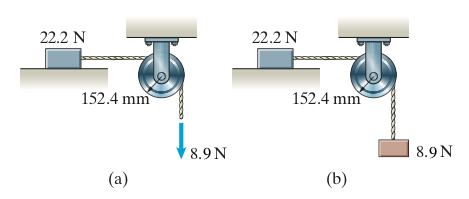
\includegraphics{./BF18_17.png}
\caption{BlockTalja}
\end{figure}

    \hypertarget{luxf6sning}{%
\section{Lösning:}\label{luxf6sning}}

    \hypertarget{friluxe4ggning-och-krafter}{%
\subsection{Friläggning och krafter}\label{friluxe4ggning-och-krafter}}

För att lösa de två fallen behöver vi frilägga systemen. Först inför vi
följande beteckningar för (a)-uppgiften

\begin{figure}
\centering
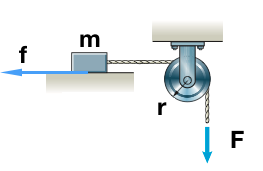
\includegraphics{./BF18_17a.png}
\caption{LabelA}
\end{figure}

samt för (b)-uppgiften.

\begin{figure}
\centering
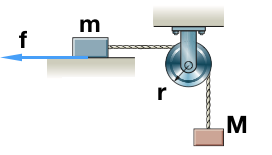
\includegraphics{./BF18_17b.png}
\caption{LabelB}
\end{figure}

Därefter kan vi frilägga de individuella delsystemen enligt nedan.

Den glidande massan \(m\) 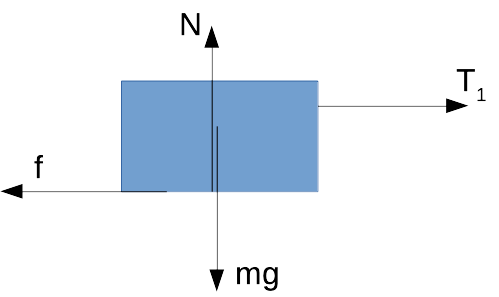
\includegraphics{./BF18_17mf.png} där
\begin{align}
&\mathbf{f} =-f\hat{x}=\mu_k N \hat{x} \\
&\mathbf{T}_1 =T_1\hat{x} \\
&\mathbf{N} =N\hat{y} \\
&m\mathbf{g} =-mg\hat{y}
\end{align}

Den roterande trissan \(s\) 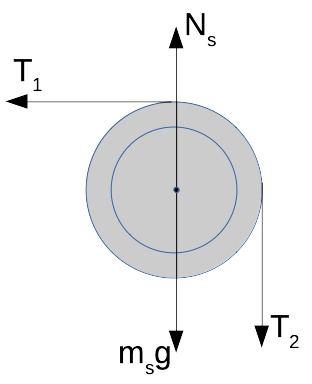
\includegraphics{./BF18_17sf.png} där
\begin{align}
&\mathbf{T}_1 =-T_1\hat{x} \\
&\mathbf{N}_s =N_s\hat{y} \\
&m_s\mathbf{g} =-m_sg\hat{y} \\
&\mathbf{T}_2 =T_2\hat{y}
\end{align}

Den fallande massan \(M\) 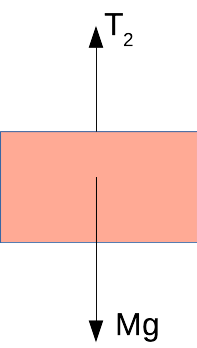
\includegraphics{./BF18_17mmf.png} där
\begin{align}
&\mathbf{T}_2 =T_2\hat{y} \\
&M\mathbf{g} =-Mg\hat{y}
\end{align}

I samtliga figurer ansätter vi ett koordinatsystem med \(x\)-axeln åt
höger och \(y\) uppåt.

    \hypertarget{fysikaliska-samband}{%
\subsection{Fysikaliska samband}\label{fysikaliska-samband}}

Med alla delsystem frilagda kan vi ställa upp Euler I och Euler II där
det är relevant. Här kan antas att massan \(m\) rör sig i \(x\)-led men
inte roterar och trissan \(s\) roterar men att dess masscentrum inte
accelererar. I uppgift (b) kan massan \(M\) röra sig i \(y\)-led.

Kopplingen mellan rörelsekvationerna för de individuella systemen görs
sedan genom snörkrafterna där det för ett masslöst snöre gäller att
snörkraften är lika stor i båda riktningar. Därför använder vi \(T_1\) i
friläggningarna för både massan \(m\) och trissan.

Utöver Euler I och Euler II har vi även kinematiska tvångsvillkor där
\(a_m=a_M\) och \(a_m=-\alpha r\) eftersom snöret inte är töjbart.
Minustecknet i rullvillkoret kommer från att vi ansätter
\(\mathbf{a}_m=a_m\hat{x}\) och \(\alpha=\alpha\hat{z}\).

    \hypertarget{kraft--och-momentanalys-euler-i-och-ii}{%
\subsection{Kraft- och momentanalys: Euler I och
II}\label{kraft--och-momentanalys-euler-i-och-ii}}

\hypertarget{massan-m}{%
\paragraph{Massan m}\label{massan-m}}

Euler I för massan m:
\(\sum_i \mathbf{F}_i = \mathbf{T}_1 + m\mathbf{g} + \mathbf{N} + \mathbf{f} = m\mathbf{a}\)

Komposantuppdelning i \(\hat{x}\)- och \(\hat{y}\)-led av verkande
krafter gör att vi kan formulera Euler I i vardera riktning.

\(\hat{x}\): \(T_1-f= T_1-\mu N= ma_m\) \textbf{(I)}

\(\hat{y}\): \(N - mg = 0\) \textbf{(II)}

\hypertarget{trissan}{%
\paragraph{Trissan}\label{trissan}}

Euler II för trissan:
\(\sum_i \mathbf{M}^P_i = \sum_i \mathbf{r}_i \times \mathbf{F}_i = I\alpha\).
Ett bra val av momentpunkt är här trissans upphängningspunkt för då ger
inte \(\mathbf{N}_s\) och \(m_s\mathbf{g}\) upphov till några
kraftmoment. Då kan vi skriva

\(\sum_i \mathbf{M} = \sum_i \mathbf{r}_i \times \mathbf{F}_i = \mathbf{r}_1 \times \mathbf{T}_1 + \mathbf{r}_2 \times \mathbf{T}_2\)

Vektorerna \(\mathbf{r}_1\) och \(\mathbf{r}_2\) kan från figurerna ovan
bestämmas till

\(\mathbf{r}_1 = r \hat{y} \\ \mathbf{r}_2 = r \hat{x}\)

så att alla kraftmoment ligger i \(z\)-riktningen:

\(\sum_i \mathbf{M} = r\hat{y} \times (-T_1\hat{x}) + r\hat{x} \times (-T_2 \hat{y}) = T_1 r - T_2 r = I\alpha\)
\textbf{(III)}

\hypertarget{massan-m-1}{%
\paragraph{Massan M}\label{massan-m-1}}

Euler I för massan M: $\sum\_i \mathbf{F}_i = \mathbf{T}_2 + M\mathbf{g}$

Komposantuppdelning i \(\hat{x}\)- och \(\hat{y}\)-led av verkande
krafter gör att vi kan formulera Euler I i vardera riktning.

\(\hat{y}\): \(T_2 - Mg = Ma_M\) \textbf{(IV)}

    \hypertarget{ekvationsluxf6sning-fuxf6r-uppgift-a}{%
\subsection{Ekvationslösning för uppgift
(a)}\label{ekvationsluxf6sning-fuxf6r-uppgift-a}}

Från \textbf{(II)} fås att \(N=mg\) vilket ger att
\(f=\mu_k N = \mu_k mg\) vilket insatt i \textbf{(I)} ger

\(T_1-\mu_k mg = ma_m\)

Här kan \(T_1\) lösas ut. För uppgift (a) är \(T_2=F\) vilket gör att vi
kan skriva \textbf{(III)} som

\(I\alpha = (m a_m+\mu_k mg) r - Fr\) \textbf{(V)}

där vi sedan kan sätta in rullvillkoret \(-m_a=r\alpha\) så att

\begin{align}
-I\frac{a_m}{r} &= (m a_m+\mu_k mg) r - Fr \\
-I\frac{a_m}{r} &= (m a_m+\mu_k mg) r - Fr \\
-I\frac{a_m}{r^2} &= m a_m+\mu_k mg - F \\
 m a_m+I\frac{a_m}{r^2} &= F-\mu_k mg \\
 a_m(m+\frac{I}{r^2}) &= F-\mu_k mg \\
 a_m &= \frac{F-\mu_k mg}{m+\frac{I}{r^2}}
\end{align}
vilket ger svaret i (a).

    \hypertarget{ekvationsluxf6sning-fuxf6r-uppgift-b}{%
\subsection{Ekvationslösning för uppgift
(b)}\label{ekvationsluxf6sning-fuxf6r-uppgift-b}}

Uppgift (b) kan lösas på ett liknande sätt förutom att här är
snörkraften \(T_2\) inte \(F\) som i uppgift (a), utan \(T_2\) måste
beräknas från Euler I för massan M.

Från \textbf{(IV)} fås att \(T_2=Mg-Ma_M\) vilket kan sättas in istället
för \(F\) i \textbf{(V)} så att

\(I\alpha = (m a_m+\mu_k mg) r - (Mg-Ma_M)r\) \textbf{(VI)}

där vi sedan kan sätta in rullvillkoret \(-m_a=r\alpha\) och dessutom
införa \(a=a_m=a_M\) så att

\begin{align}
-&I\frac{a}{r} = (m a+\mu_k mg) r - (Mg-Ma)r \\
-&I\frac{a}{r} = (m a+\mu_k mg) r - (Mg-Ma)r \\
-&I\frac{a}{r^2} = m a+\mu_k mg - (Mg-Ma) \\
& m a + M a +I\frac{a_m}{r^2} = Mg -\mu_k mg \\
& a (m+M+\frac{I}{r^2}) = Mg-\mu_k mg \\
& a = \frac{Mg-\mu_k mg}{m+M+\frac{I}{r^2}}
\end{align}
vilket ger svaret i (b).

    \hypertarget{svar}{%
\subsection{Svar}\label{svar}}

Med insatta värden blir \(a_m=a=0.1748~m/s^2\) för uppgift (a) och
\(a_m=a=0.1688~m/s^2\) för uppgift (b).

    \hypertarget{analys}{%
\subsection{Analys}\label{analys}}

Trots att uppgifterna ser snarlika ut blir accelerationen i (b) lägre.
Det beror på att den ändliga massan M i (b) gör att snörkraften \(T_2\)
blir mindre än i (a). Det kan ses som att utöver att få trissan att
snurra så behöver kraften på 8.9 N accelerera både M och m i (b) men
bara m i (a).

Notera också att \(T_1\neq T_2\) här. Det kan vara ovant från tidigare
kurser där snörkraften typiskt är konstant över hela snörets längd. Men
det beror ju på att snöret då anses masslöst. Här, och i liknande
trissa-uppgifter har vi dock en ändlig tröghetstensor \(I\) för trissan
så även om snöret är fortsatt masslöst visar Euler II att snörkrafterna
är olika stora.

    \textbf{Beräkning med insatta värden:}

    \begin{tcolorbox}[breakable, size=fbox, boxrule=1pt, pad at break*=1mm,colback=cellbackground, colframe=cellborder]
\prompt{In}{incolor}{8}{\boxspacing}
\begin{Verbatim}[commandchars=\\\{\}]
\PY{k+kn}{from} \PY{n+nn}{ipywidgets} \PY{k+kn}{import} \PY{n}{interact}\PY{p}{,} \PY{n}{interactive}
\PY{k+kn}{from} \PY{n+nn}{ipywidgets} \PY{k+kn}{import} \PY{n}{FloatSlider}
\PY{k+kn}{import} \PY{n+nn}{numpy} \PY{k}{as} \PY{n+nn}{np}
\PY{k+kn}{from} \PY{n+nn}{IPython}\PY{n+nn}{.}\PY{n+nn}{display} \PY{k+kn}{import} \PY{n}{HTML}
\end{Verbatim}
\end{tcolorbox}

    \begin{tcolorbox}[breakable, size=fbox, boxrule=1pt, pad at break*=1mm,colback=cellbackground, colframe=cellborder]
\prompt{In}{incolor}{9}{\boxspacing}
\begin{Verbatim}[commandchars=\\\{\}]
\PY{n}{HTML}\PY{p}{(}\PY{l+s+s1}{\PYZsq{}\PYZsq{}\PYZsq{}}\PY{l+s+s1}{\PYZlt{}script\PYZgt{}}
\PY{l+s+s1}{code\PYZus{}show=true; }
\PY{l+s+s1}{function code\PYZus{}toggle() }\PY{l+s+s1}{\PYZob{}}
\PY{l+s+s1}{ if (code\PYZus{}show)}\PY{l+s+s1}{\PYZob{}}
\PY{l+s+s1}{ \PYZdl{}(}\PY{l+s+s1}{\PYZsq{}}\PY{l+s+s1}{div.input}\PY{l+s+s1}{\PYZsq{}}\PY{l+s+s1}{).hide();}
\PY{l+s+s1}{ \PYZcb{} else }\PY{l+s+s1}{\PYZob{}}
\PY{l+s+s1}{ \PYZdl{}(}\PY{l+s+s1}{\PYZsq{}}\PY{l+s+s1}{div.input}\PY{l+s+s1}{\PYZsq{}}\PY{l+s+s1}{).show();}
\PY{l+s+s1}{ \PYZcb{}}
\PY{l+s+s1}{ code\PYZus{}show = !code\PYZus{}show}
\PY{l+s+s1}{\PYZcb{} }
\PY{l+s+s1}{\PYZdl{}( document ).ready(code\PYZus{}toggle);}
\PY{l+s+s1}{\PYZlt{}/script\PYZgt{}}
\PY{l+s+s1}{\PYZlt{}form action=}\PY{l+s+s1}{\PYZdq{}}\PY{l+s+s1}{javascript:code\PYZus{}toggle()}\PY{l+s+s1}{\PYZdq{}}\PY{l+s+s1}{\PYZgt{}\PYZlt{}input type=}\PY{l+s+s1}{\PYZdq{}}\PY{l+s+s1}{submit}\PY{l+s+s1}{\PYZdq{}}\PY{l+s+s1}{ value=}\PY{l+s+s1}{\PYZdq{}}\PY{l+s+s1}{Tryck här för att dölja/visa koden.}\PY{l+s+s1}{\PYZdq{}}\PY{l+s+s1}{\PYZgt{}\PYZlt{}/form\PYZgt{}}\PY{l+s+s1}{\PYZsq{}\PYZsq{}\PYZsq{}}\PY{p}{)}
\end{Verbatim}
\end{tcolorbox}

            \begin{tcolorbox}[breakable, size=fbox, boxrule=.5pt, pad at break*=1mm, opacityfill=0]
\prompt{Out}{outcolor}{9}{\boxspacing}
\begin{Verbatim}[commandchars=\\\{\}]
<IPython.core.display.HTML object>
\end{Verbatim}
\end{tcolorbox}
        
    \begin{tcolorbox}[breakable, size=fbox, boxrule=1pt, pad at break*=1mm,colback=cellbackground, colframe=cellborder]
\prompt{In}{incolor}{10}{\boxspacing}
\begin{Verbatim}[commandchars=\\\{\}]
\PY{c+c1}{\PYZsh{} Set parameters according to exercise description}

\PY{n}{G} \PY{o}{=} \PY{l+m+mf}{9.81}  \PY{c+c1}{\PYZsh{} acceleration due to gravity, in m/s\PYZca{}2}

\PY{n}{mu} \PY{o}{=} \PY{l+m+mf}{0.22}
\PY{n}{mg}\PY{o}{=}\PY{l+m+mf}{22.2}
\PY{n}{I}\PY{o}{=}\PY{l+m+mf}{0.54}
\PY{n}{r}\PY{o}{=}\PY{l+m+mf}{0.1524}
\PY{n}{F}\PY{o}{=}\PY{l+m+mf}{8.9}
\end{Verbatim}
\end{tcolorbox}

    \begin{tcolorbox}[breakable, size=fbox, boxrule=1pt, pad at break*=1mm,colback=cellbackground, colframe=cellborder]
\prompt{In}{incolor}{11}{\boxspacing}
\begin{Verbatim}[commandchars=\\\{\}]
\PY{k}{def} \PY{n+nf}{e\PYZus{}18\PYZus{}17a}\PY{p}{(}\PY{n}{F}\PY{p}{,}\PY{n}{mu}\PY{p}{,}\PY{n}{mg}\PY{p}{,}\PY{n}{I}\PY{p}{)}\PY{p}{:}

    \PY{n}{m}\PY{o}{=}\PY{n}{mg}\PY{o}{/}\PY{n}{G}
    \PY{n}{m2}\PY{o}{=}\PY{n}{F}\PY{o}{/}\PY{n}{G}
    \PY{n}{a\PYZus{}a}\PY{o}{=}\PY{n+nb}{max}\PY{p}{(}\PY{l+m+mf}{0.0}\PY{p}{,}\PY{p}{(}\PY{n}{F}\PY{o}{\PYZhy{}}\PY{n}{mu}\PY{o}{*}\PY{n}{mg}\PY{p}{)}\PY{o}{/}\PY{p}{(}\PY{n}{m}\PY{o}{+}\PY{n}{I}\PY{o}{/}\PY{n}{r}\PY{o}{*}\PY{o}{*}\PY{l+m+mi}{2}\PY{p}{)}\PY{p}{)}

    \PY{n+nb}{print}\PY{p}{(}\PY{l+s+s2}{\PYZdq{}}\PY{l+s+s2}{Accelerationen a i uppgift (a)= }\PY{l+s+s2}{\PYZdq{}}\PY{p}{,}\PY{l+s+s1}{\PYZsq{}}\PY{l+s+si}{\PYZob{}:5.3f\PYZcb{}}\PY{l+s+s1}{\PYZsq{}}\PY{o}{.}\PY{n}{format}\PY{p}{(}\PY{n}{a\PYZus{}a}\PY{p}{)}\PY{p}{,}\PY{l+s+s2}{\PYZdq{}}\PY{l+s+s2}{m/s\PYZca{}2}\PY{l+s+s2}{\PYZdq{}}\PY{p}{)}



    \PY{k}{return} \PY{n}{a\PYZus{}a}
\end{Verbatim}
\end{tcolorbox}

    \begin{tcolorbox}[breakable, size=fbox, boxrule=1pt, pad at break*=1mm,colback=cellbackground, colframe=cellborder]
\prompt{In}{incolor}{12}{\boxspacing}
\begin{Verbatim}[commandchars=\\\{\}]
\PY{k}{def} \PY{n+nf}{e\PYZus{}18\PYZus{}17b}\PY{p}{(}\PY{n}{mu}\PY{p}{,}\PY{n}{mg}\PY{p}{,}\PY{n}{Mg}\PY{p}{,}\PY{n}{I}\PY{p}{)}\PY{p}{:}

    \PY{n}{m}\PY{o}{=}\PY{n}{mg}\PY{o}{/}\PY{n}{G}
    \PY{n}{m2}\PY{o}{=}\PY{n}{Mg}\PY{o}{/}\PY{n}{G}
    \PY{n}{a\PYZus{}b}\PY{o}{=}\PY{n+nb}{max}\PY{p}{(}\PY{l+m+mf}{0.0}\PY{p}{,}\PY{p}{(}\PY{n}{F}\PY{o}{\PYZhy{}}\PY{n}{mu}\PY{o}{*}\PY{n}{mg}\PY{p}{)}\PY{o}{/}\PY{p}{(}\PY{n}{m}\PY{o}{+}\PY{n}{m2}\PY{o}{+}\PY{n}{I}\PY{o}{/}\PY{n}{r}\PY{o}{*}\PY{o}{*}\PY{l+m+mi}{2}\PY{p}{)}\PY{p}{)}

    \PY{n+nb}{print}\PY{p}{(}\PY{l+s+s2}{\PYZdq{}}\PY{l+s+s2}{Accelerationen a i uppgift (b)= }\PY{l+s+s2}{\PYZdq{}}\PY{p}{,}\PY{l+s+s1}{\PYZsq{}}\PY{l+s+si}{\PYZob{}:5.3f\PYZcb{}}\PY{l+s+s1}{\PYZsq{}}\PY{o}{.}\PY{n}{format}\PY{p}{(}\PY{n}{a\PYZus{}b}\PY{p}{)}\PY{p}{,}\PY{l+s+s2}{\PYZdq{}}\PY{l+s+s2}{m/s\PYZca{}2}\PY{l+s+s2}{\PYZdq{}}\PY{p}{)}



    \PY{k}{return} \PY{n}{a\PYZus{}b}
\end{Verbatim}
\end{tcolorbox}

    \begin{tcolorbox}[breakable, size=fbox, boxrule=1pt, pad at break*=1mm,colback=cellbackground, colframe=cellborder]
\prompt{In}{incolor}{13}{\boxspacing}
\begin{Verbatim}[commandchars=\\\{\}]
\PY{n}{s\PYZus{}18\PYZus{}17a}\PY{o}{=}\PY{n}{interactive}\PY{p}{(}\PY{n}{e\PYZus{}18\PYZus{}17a}\PY{p}{,} 
              \PY{n}{F}\PY{o}{=}\PY{n}{FloatSlider}\PY{p}{(}\PY{n+nb}{min}\PY{o}{=}\PY{l+m+mf}{0.0}\PY{p}{,}\PY{n+nb}{max}\PY{o}{=}\PY{l+m+mi}{20}\PY{p}{,}\PY{n}{value}\PY{o}{=}\PY{l+m+mf}{8.9}\PY{p}{)}\PY{p}{,}
              \PY{n}{mu}\PY{o}{=}\PY{n}{FloatSlider}\PY{p}{(}\PY{n+nb}{min}\PY{o}{=}\PY{l+m+mf}{0.0}\PY{p}{,}\PY{n+nb}{max}\PY{o}{=}\PY{l+m+mf}{0.40}\PY{p}{,}\PY{n}{value}\PY{o}{=}\PY{l+m+mf}{0.22}\PY{p}{,}\PY{n}{step}\PY{o}{=}\PY{l+m+mf}{0.01}\PY{p}{)}\PY{p}{,}
              \PY{n}{mg}\PY{o}{=}\PY{n}{FloatSlider}\PY{p}{(}\PY{n+nb}{min}\PY{o}{=}\PY{l+m+mf}{0.0}\PY{p}{,}\PY{n+nb}{max}\PY{o}{=}\PY{l+m+mf}{40.0}\PY{p}{,}\PY{n}{value}\PY{o}{=}\PY{l+m+mf}{22.2}\PY{p}{,}\PY{n}{step}\PY{o}{=}\PY{l+m+mf}{0.01}\PY{p}{)}\PY{p}{,}
              \PY{n}{I}\PY{o}{=}\PY{n}{FloatSlider}\PY{p}{(}\PY{n+nb}{min}\PY{o}{=}\PY{l+m+mf}{0.0}\PY{p}{,}\PY{n+nb}{max}\PY{o}{=}\PY{l+m+mf}{1.0}\PY{p}{,}\PY{n}{value}\PY{o}{=}\PY{l+m+mf}{0.54}\PY{p}{,}\PY{n}{step}\PY{o}{=}\PY{l+m+mf}{0.01}\PY{p}{)}\PY{p}{,}\PY{p}{)}
\PY{n}{display}\PY{p}{(}\PY{n}{s\PYZus{}18\PYZus{}17a}\PY{p}{)}
\end{Verbatim}
\end{tcolorbox}

    
    \begin{Verbatim}[commandchars=\\\{\}]
interactive(children=(FloatSlider(value=8.9, description='F', max=20.0), FloatSlider(value=0.22, description='…
    \end{Verbatim}

    
    \begin{tcolorbox}[breakable, size=fbox, boxrule=1pt, pad at break*=1mm,colback=cellbackground, colframe=cellborder]
\prompt{In}{incolor}{ }{\boxspacing}
\begin{Verbatim}[commandchars=\\\{\}]
\PY{n}{s\PYZus{}18\PYZus{}17b}\PY{o}{=}\PY{n}{interactive}\PY{p}{(}\PY{n}{e\PYZus{}18\PYZus{}17b}\PY{p}{,} 
              \PY{n}{mu}\PY{o}{=}\PY{n}{FloatSlider}\PY{p}{(}\PY{n+nb}{min}\PY{o}{=}\PY{l+m+mf}{0.0}\PY{p}{,}\PY{n+nb}{max}\PY{o}{=}\PY{l+m+mf}{0.40}\PY{p}{,}\PY{n}{value}\PY{o}{=}\PY{l+m+mf}{0.22}\PY{p}{,}\PY{n}{step}\PY{o}{=}\PY{l+m+mf}{0.01}\PY{p}{)}\PY{p}{,}
              \PY{n}{mg}\PY{o}{=}\PY{n}{FloatSlider}\PY{p}{(}\PY{n+nb}{min}\PY{o}{=}\PY{l+m+mf}{0.0}\PY{p}{,}\PY{n+nb}{max}\PY{o}{=}\PY{l+m+mf}{40.0}\PY{p}{,}\PY{n}{value}\PY{o}{=}\PY{l+m+mf}{22.2}\PY{p}{,}\PY{n}{step}\PY{o}{=}\PY{l+m+mf}{0.01}\PY{p}{)}\PY{p}{,}
              \PY{n}{Mg}\PY{o}{=}\PY{n}{FloatSlider}\PY{p}{(}\PY{n+nb}{min}\PY{o}{=}\PY{l+m+mf}{0.0}\PY{p}{,}\PY{n+nb}{max}\PY{o}{=}\PY{l+m+mf}{20.0}\PY{p}{,}\PY{n}{value}\PY{o}{=}\PY{l+m+mf}{8.9}\PY{p}{,}\PY{n}{step}\PY{o}{=}\PY{l+m+mf}{0.01}\PY{p}{)}\PY{p}{,}
              \PY{n}{I}\PY{o}{=}\PY{n}{FloatSlider}\PY{p}{(}\PY{n+nb}{min}\PY{o}{=}\PY{l+m+mf}{0.0}\PY{p}{,}\PY{n+nb}{max}\PY{o}{=}\PY{l+m+mf}{1.0}\PY{p}{,}\PY{n}{value}\PY{o}{=}\PY{l+m+mf}{0.54}\PY{p}{,}\PY{n}{step}\PY{o}{=}\PY{l+m+mf}{0.01}\PY{p}{)}\PY{p}{,}\PY{p}{)}
\PY{n}{display}\PY{p}{(}\PY{n}{s\PYZus{}18\PYZus{}17b}\PY{p}{)}
\end{Verbatim}
\end{tcolorbox}

    \begin{tcolorbox}[breakable, size=fbox, boxrule=1pt, pad at break*=1mm,colback=cellbackground, colframe=cellborder]
\prompt{In}{incolor}{ }{\boxspacing}
\begin{Verbatim}[commandchars=\\\{\}]

\end{Verbatim}
\end{tcolorbox}


    % Add a bibliography block to the postdoc
    
    
    
\end{document}
